\documentclass[UTF8,12pt,fontset=fandol]{ctexart}

\usepackage[a4paper,top=3.5cm,bottom=2.6cm,left=3cm,right=2.6cm]{geometry}
\usepackage{fontspec}
\usepackage{xeCJK}
\usepackage{setspace}
\usepackage{indentfirst}
\usepackage{graphicx}
\usepackage{caption}
\usepackage{subcaption}
\usepackage{booktabs}
\usepackage{amsmath}
\usepackage{amssymb}
\usepackage{longtable}
\usepackage{array}
\usepackage{float}
\usepackage{hyperref}
\usepackage{fancyhdr}

\setmainfont{Times New Roman}
\IfFontExistsTF{Songti SC}{
    \setCJKmainfont{Songti SC}
}{
    \setCJKmainfont{FandolSong-Regular}
}
\IfFontExistsTF{Heiti SC}{
    \setCJKsansfont{Heiti SC}
}{
    \setCJKsansfont{FandolHei-Regular}
}

\setlength{\parindent}{2em}
\setlength{\parskip}{0pt}
\AtBeginDocument{\fontsize{12bp}{22bp}\selectfont}

\pagestyle{fancy}
\fancyhf{}
\fancyfoot[C]{\thepage}
\renewcommand{\headrulewidth}{0pt}
\setlength{\headheight}{12pt}
\setlength{\footskip}{2.0cm}

\DeclareCaptionFont{bitcapfont}{\CJKfamily{\CJKrmdefault}\zihao{5}}
\captionsetup[figure]{font=bitcapfont,labelfont=bitcapfont,labelsep=space}


\newcommand{\hfirst}[1]{%
\vspace{0.6em}
\noindent\textbf{#1}\par
}

\newcommand{\subh}[1]{%
\vspace{0.4em}
\noindent\textbf{#1}\par
}

\begin{document}

\begin{titlepage}
    \thispagestyle{empty}
    \begin{center}
        \vspace*{1.0cm}
        {\zihao{2}\bfseries 本科生毕业设计（论文）\par}
        \vspace{1.0cm}
        {\zihao{1}\bfseries 中期报告\par}
        \vspace{1.4cm}
        {\zihao{2}\bfseries 端到端折衍混合光学系统设计研究\par}
        \vspace{0.6cm}
        {\zihao{4}\bfseries End-to-End Hybrid Refractive-Diffractive Lens Design\par}
        \vspace{1.8cm}
    \end{center}

    \renewcommand{\arraystretch}{1.55}
    \begin{center}
    \begin{tabular}{p{3.2cm}p{8.0cm}}
        学\hspace{1.2em}院： & 光电学院 \\
        专\hspace{1.2em}业： & 测控技术与仪器 \\
        班\hspace{1.2em}级： &  0402201\\
        学生姓名： & 李俊贤 \\
        学\hspace{1.2em}号： & 1120221991 \\
        指导教师： & 张楠 \\
        日\hspace{1.2em}期： & 2026年2月7日 \\
    \end{tabular}
    \end{center}
\end{titlepage}

\clearpage
\pagenumbering{arabic}

\section*{一、毕业设计（论文）主要研究内容、进展情况及取得成果}

\hfirst{1.1 主要研究内容}
本课题围绕“大视场、小型化、高成像质量”成像系统设计需求，研究可微分射线-波动联合模型驱动的端到端折衍混合光学系统设计方法。研究内容并非单一算法实现，而是覆盖“理论建模、工程落地、对比评估、边界分析、文档可复现”五个维度，目标是在毕业设计周期内形成可验证、可复用、可解释的完整技术闭环。按照已确认路线，课题包含四条连续主线。第一条主线为纯折射系统设计，通过课程学习与微调策略建立可用基线；第二条主线为折衍混合设计，在折射基线后引入DOE参数并联合优化；第三条主线为折衍混合端到端设计，将混合光学前端与UNet后端联合训练；第四条主线为扩展研究，在主线稳定后探索折射与超表面混合设计的性能上界和工程代价。

在理论层面，本课题的核心问题是统一描述几何光学与波动光学。传统折射优化主要依赖射线追迹，而DOE或超表面的相位调制过程更适合在波动光学框架下处理。若仅使用几何近似，离轴条件下PSF预测容易偏离真实传播行为；若全流程采用高精度波动传播，计算成本又难以满足大规模迭代需求。因此，本课题采用可微分射线-波动联合建模：在折射段使用可微射线追迹保证效率，在DOE平面后采用可微衍射传播保证保真度，再将整个链路统一到自动微分框架中，以图像质量和光学质量共同驱动优化。
相关方法路径与阶段化训练思想可参考已有研究工作\cite{yang2024curriculum,yang2024endtoend}，本课题在此基础上进行工程化整合与任务适配。

在工程层面，本课题以DeepLens项目为实现基座，已形成配置层、训练层、评估层和导出层分离的模块结构。配置层负责参数统一管理，训练层负责GeoLens、HybridLens、E2E与Metasurface各阶段优化，评估层负责PSF、MTF、Spot与相位图分析，导出层负责与外部光学软件的数据接口。该工程结构的核心价值是可复现：任意一次实验都可追溯其配置、脚本、输出图和日志，从而支持论文中的可核验结论。

\hfirst{1.2 技术路线与方法框架}
课题采用“逐层递进、分段验收、统一评估”的路线，具体为“折射设计 $\rightarrow$ 折衍混合 $\rightarrow$ 端到端联合 $\rightarrow$ 超表面扩展”。这种顺序并非形式化安排，而是针对高维耦合优化问题的工程化求解策略。若在早期直接引入高自由度相位参数与重建网络参数，优化变量维数和梯度噪声都会急剧增加，训练易陷入不稳定状态。通过分阶段路线，可以在每个阶段建立局部可行解，再将其作为下阶段初始化，显著降低整体优化风险。

折射系统参数化采用偶次非球面表示，形式可写为
\begin{equation}
z(r)=\frac{cr^2}{1+\sqrt{1-(1+k)c^2r^2}}+\sum_{i=2}^{N}a_{2i}r^{2i},
\end{equation}
其中 $c$ 为曲率，$k$ 为圆锥常数，$a_{2i}$ 为高阶非球面参数。该表示兼顾表达能力和可制造性，能够覆盖多数中等复杂度光学面形优化需求。DOE调制采用相位函数 $\phi(x,y)$，入射复振幅 $U_{in}(x,y)$ 经DOE后变为
\begin{equation}
U_{doe}(x,y)=U_{in}(x,y)\exp\left(j\phi(x,y)\right),
\end{equation}
再通过菲涅尔传播得到像面场分布，PSF由像面复振幅模平方归一化获得。损失函数采用分阶段权重策略：折射阶段强调光学质量项，折衍阶段加入相位与成像联合约束，端到端阶段以PSNR为主并保留SSIM、LPIPS辅助评估。

\hfirst{1.3 参数定型原则与中期策略}
中期阶段的关键工作不是追求单次最优指标，而是建立参数定型方法。焦距、F数、厚度预算、DOE位置与分辨率共同决定优化可行域。若参数在实验中频繁变化，会导致对比不公平，结论不可核验。为此，本课题采用“粗筛+精筛”两级策略：先用低成本设置在候选区间搜索可行组合，再在统一预算下执行正式训练并固定主方案。该策略的收益在于减少盲目迭代，并为后续消融实验提供稳定基准。

就中期状态而言，参数仍处于收敛阶段，但已形成明确原则：其一，所有对比方案必须共享数据划分、训练预算与评价脚本；其二，任何参数修改必须记录版本与理由；其三，结论表达遵循“事实先行、解释随后、边界明确”，避免把未完成验证的趋势写成终局结论。

\hfirst{1.4 当前进展与阶段成果}
截至2026年2月7日，课题已完成项目框架搭建、关键脚本打通、基础评估流程建立与新一轮结果归档。当前成果目录覆盖折射结构图、MTF图、Spot图、DOE相位图、折衍混合损失曲线、端到端训练曲线、超表面扩展优化图及独立测试图，证明“折射 $\rightarrow$ 折衍混合 $\rightarrow$ 端到端 $\rightarrow$ 超表面扩展”四阶段主线均已进入可验证状态。下列图像为本轮结果中的关键证据。

\begin{figure}[H]
\centering
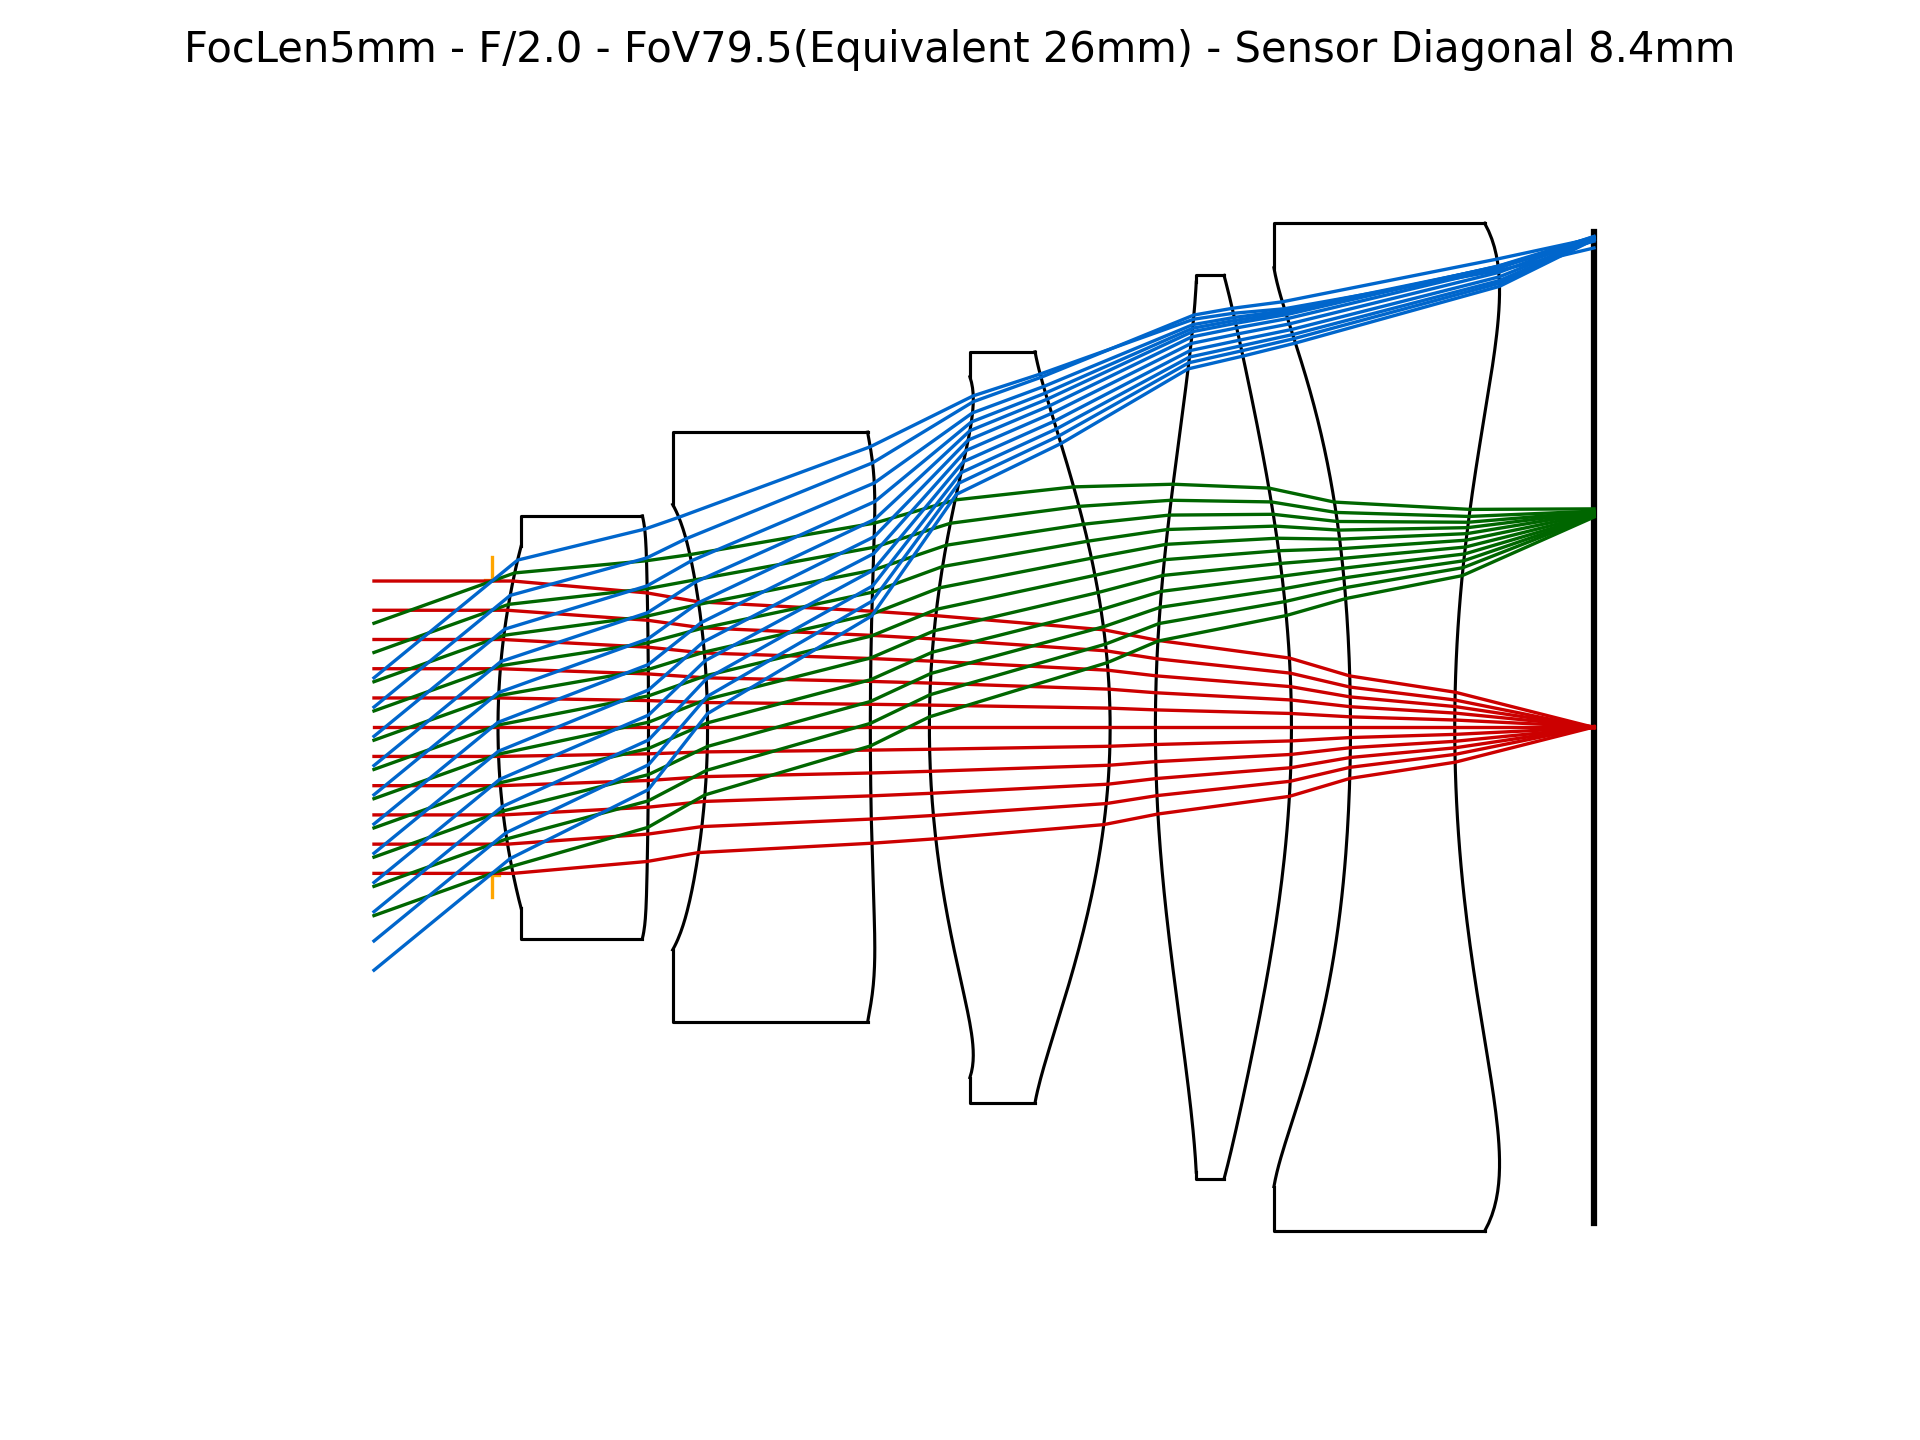
\includegraphics[width=0.78\textwidth]{figures/final_lens.png}
\caption{折射镜片结构示意（tutorial\_0207-184619）}
\end{figure}

\begin{figure}[H]
\centering
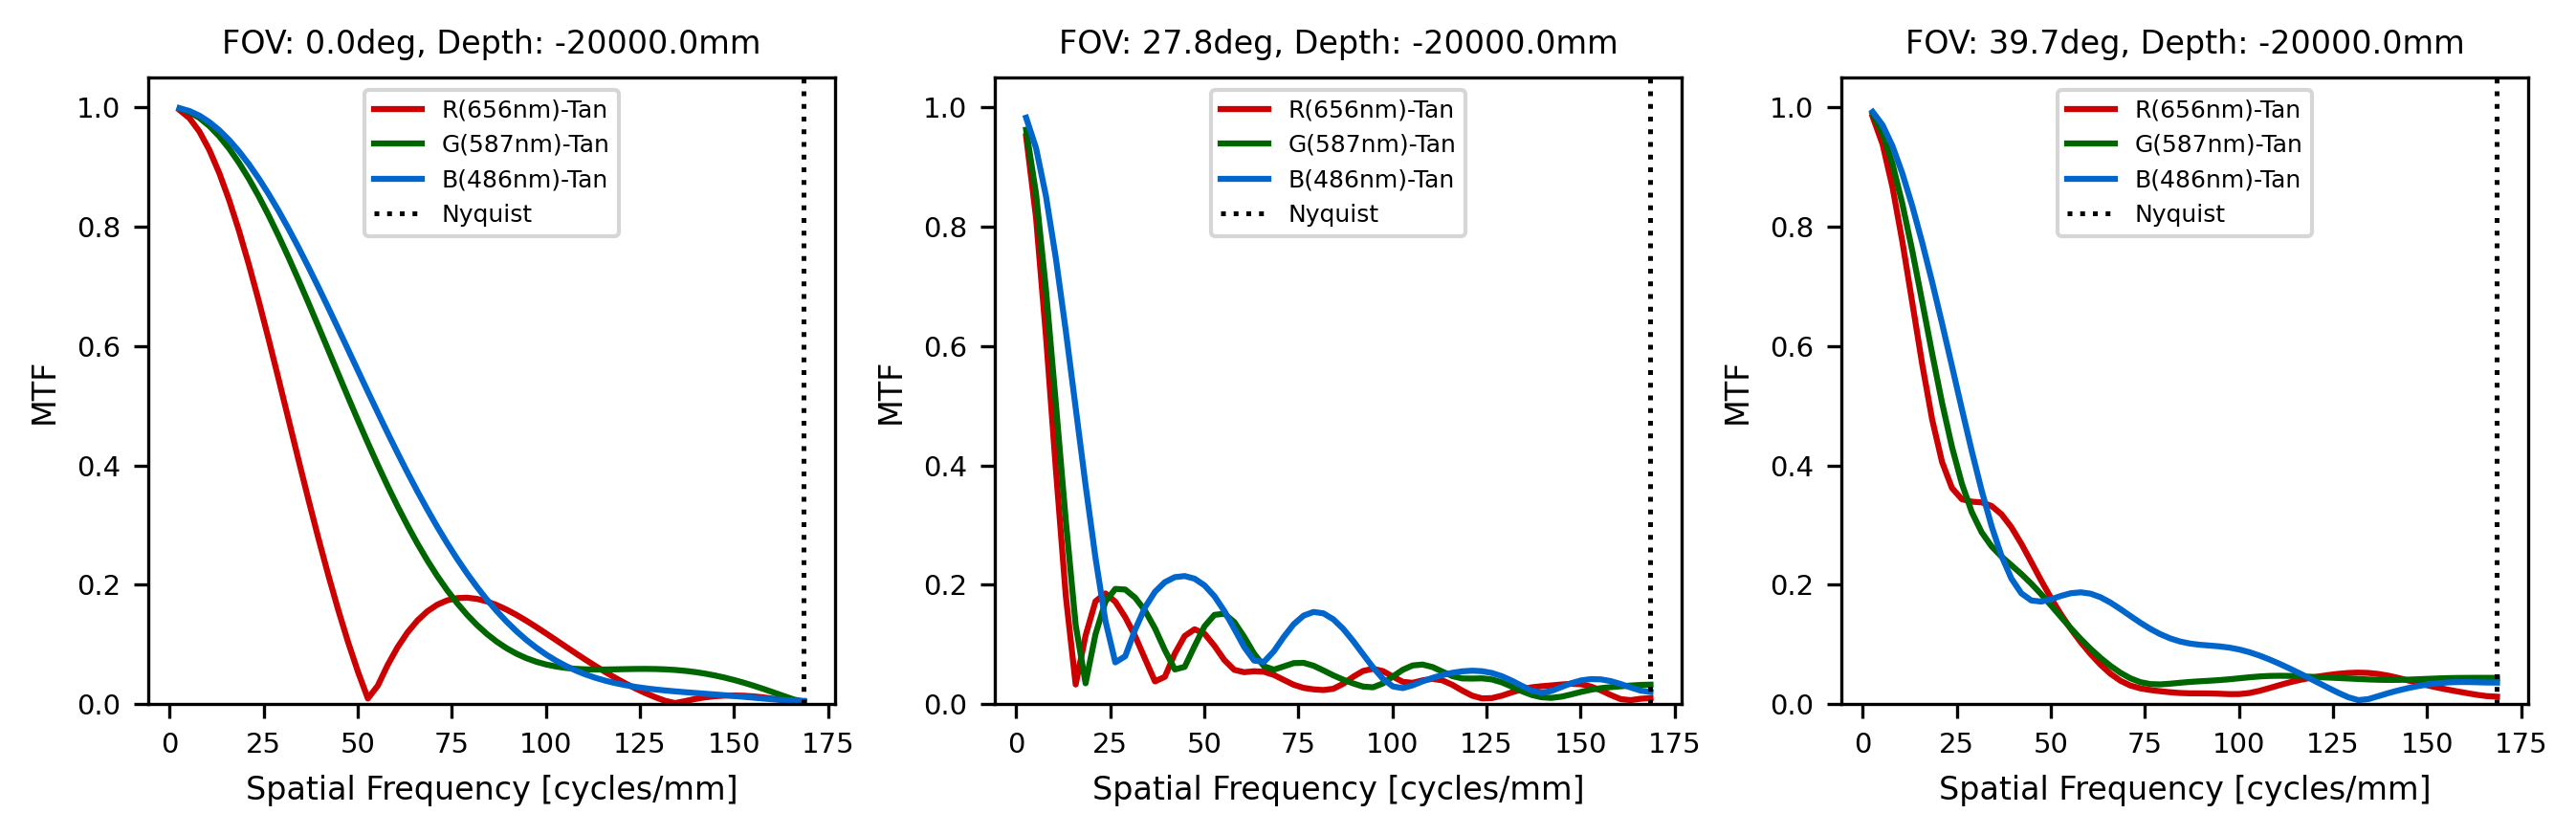
\includegraphics[width=0.78\textwidth]{figures/final_lens_mtf.png}
\caption{折射系统MTF分析图（tutorial\_0207-184619）}
\end{figure}

\begin{figure}[H]
\centering
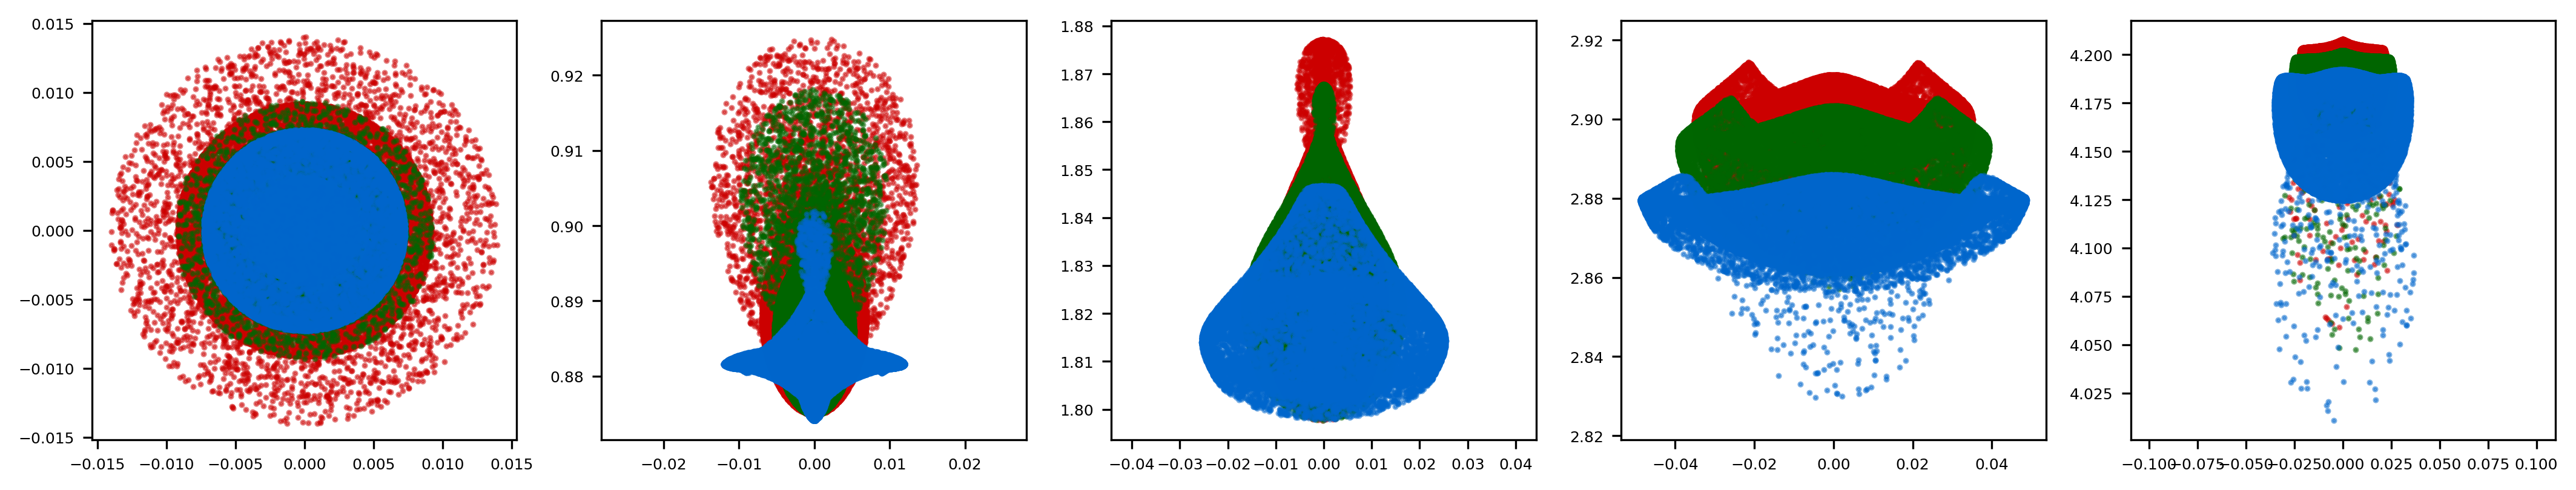
\includegraphics[width=0.78\textwidth]{figures/final_lens_spot.png}
\caption{折射系统Spot分析图（tutorial\_0207-184619）}
\end{figure}

\begin{figure}[H]
\centering
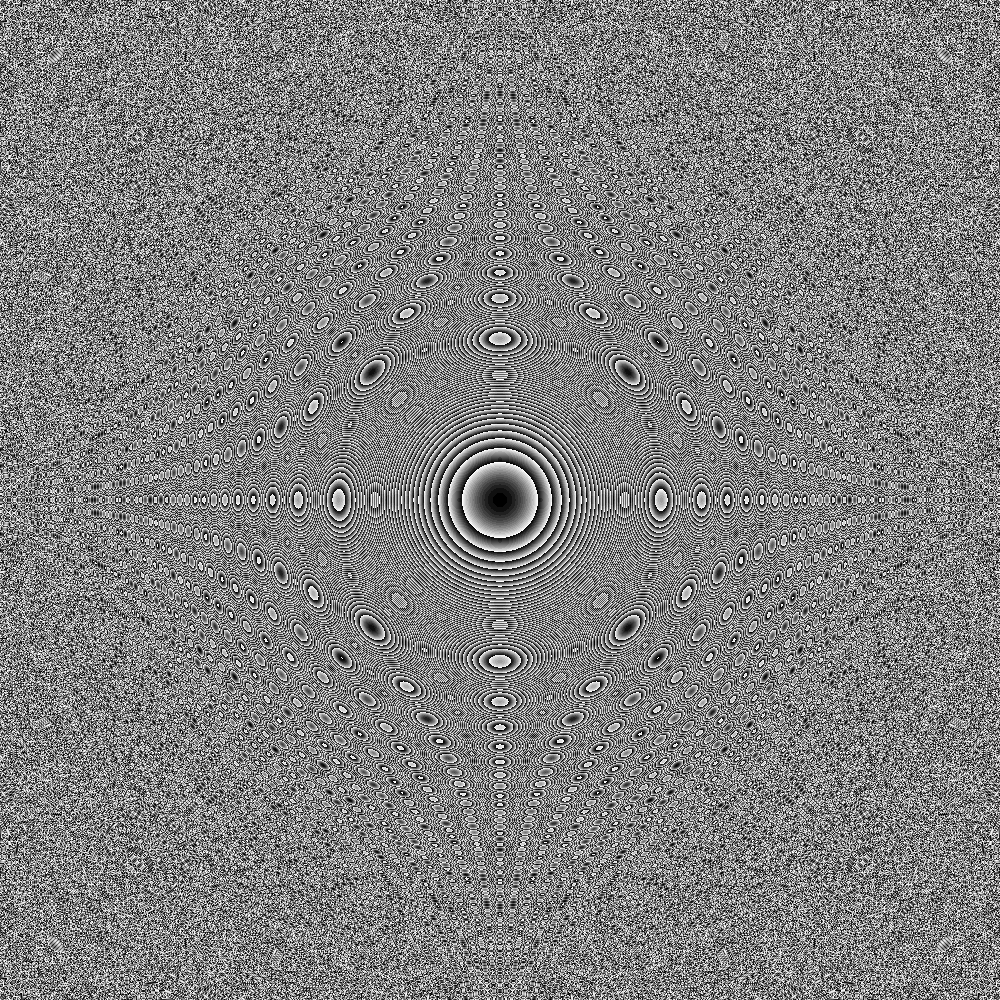
\includegraphics[width=0.78\textwidth]{figures/doe_phase_map.png}
\caption{DOE相位分布图（tutorial\_0207-184619）}
\end{figure}

\begin{figure}[H]
\centering
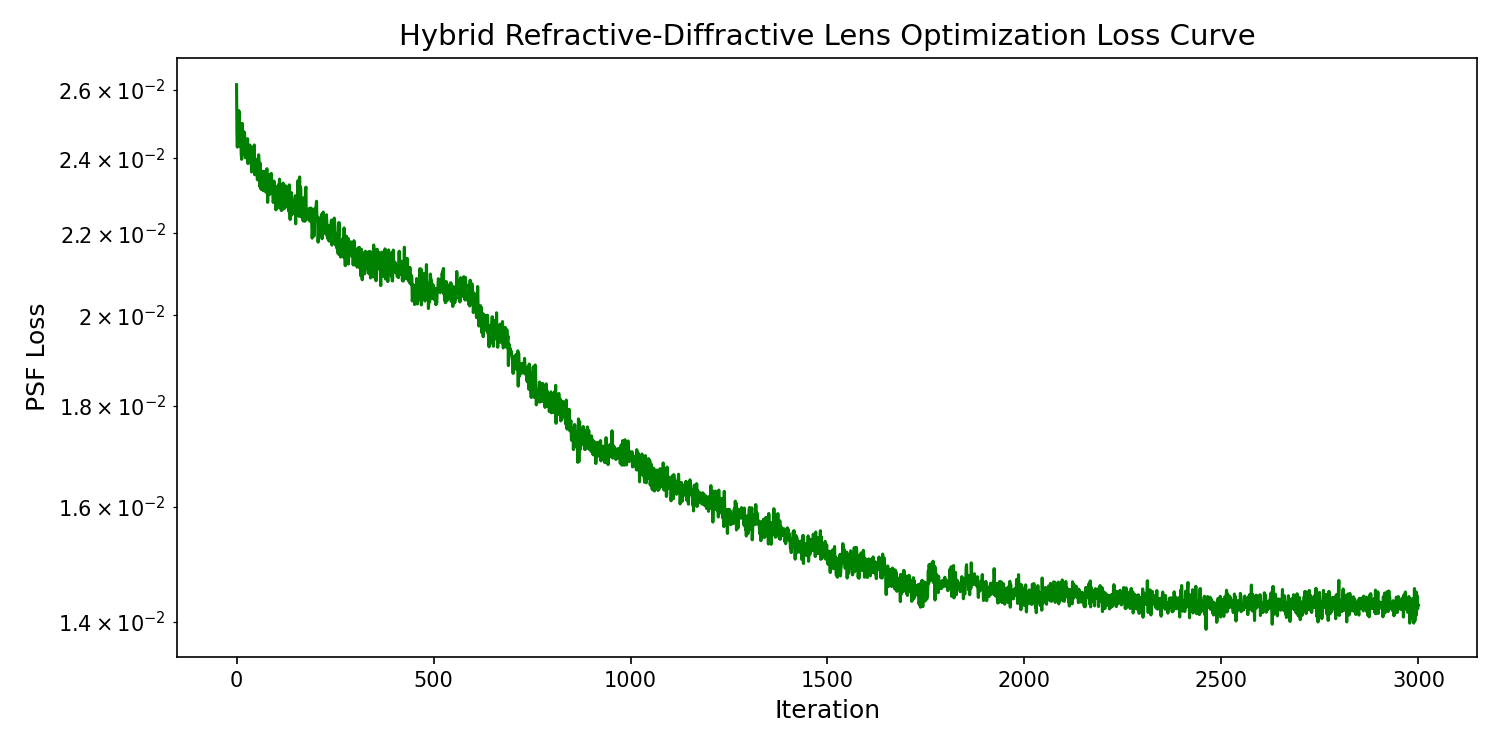
\includegraphics[width=0.78\textwidth]{figures/hybrid_loss_curve.png}
\caption{折衍混合优化损失曲线（tutorial\_0207-184619）}
\end{figure}

\begin{figure}[H]
\centering
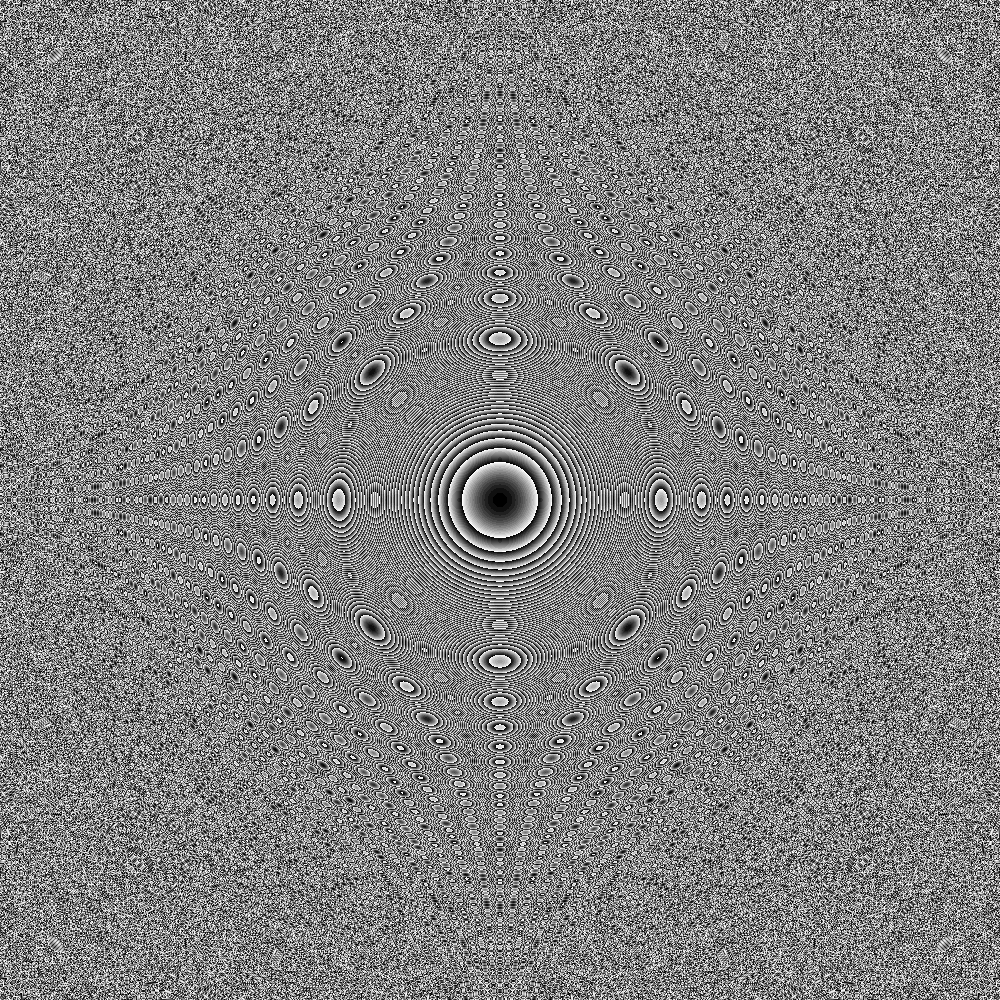
\includegraphics[width=0.78\textwidth]{figures/hybrid_final_analysis_doe.png}
\caption{折衍混合DOE分析图（tutorial\_0207-184619）}
\end{figure}

\begin{figure}[H]
\centering
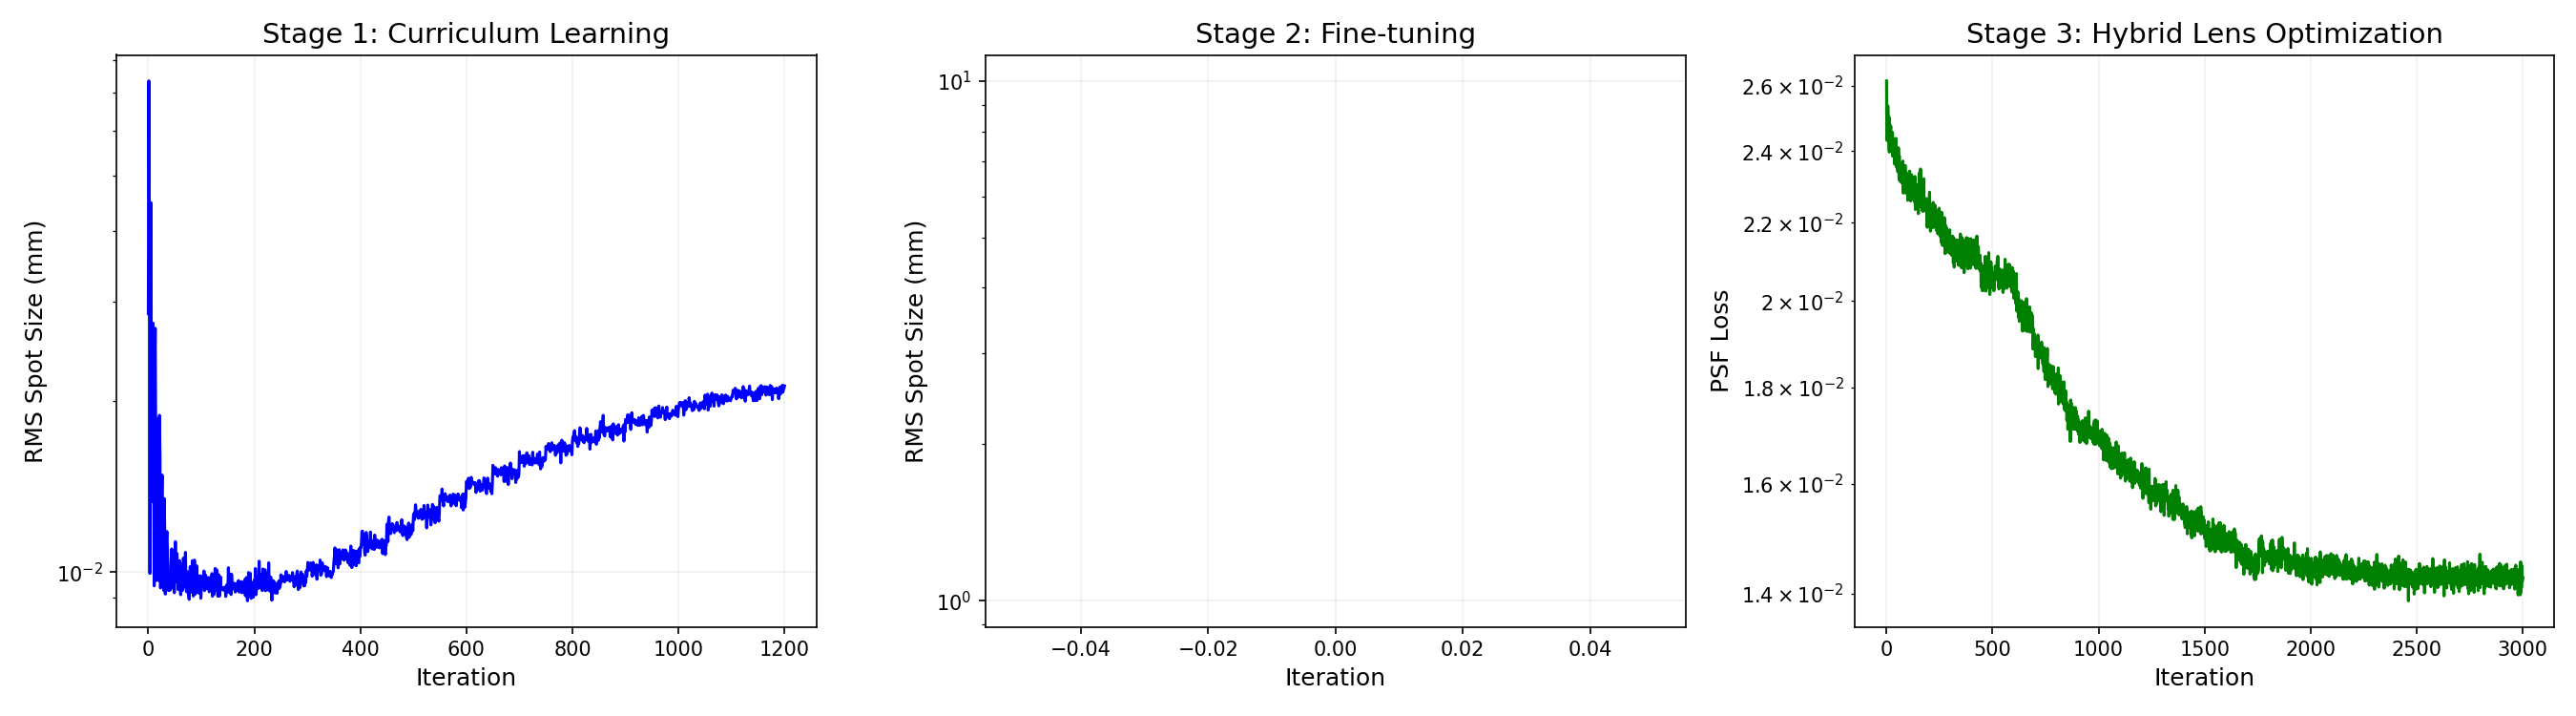
\includegraphics[width=0.78\textwidth]{figures/all_loss_curves.png}
\caption{阶段损失总览（tutorial\_0207-184619）}
\end{figure}

\begin{figure}[H]
\centering
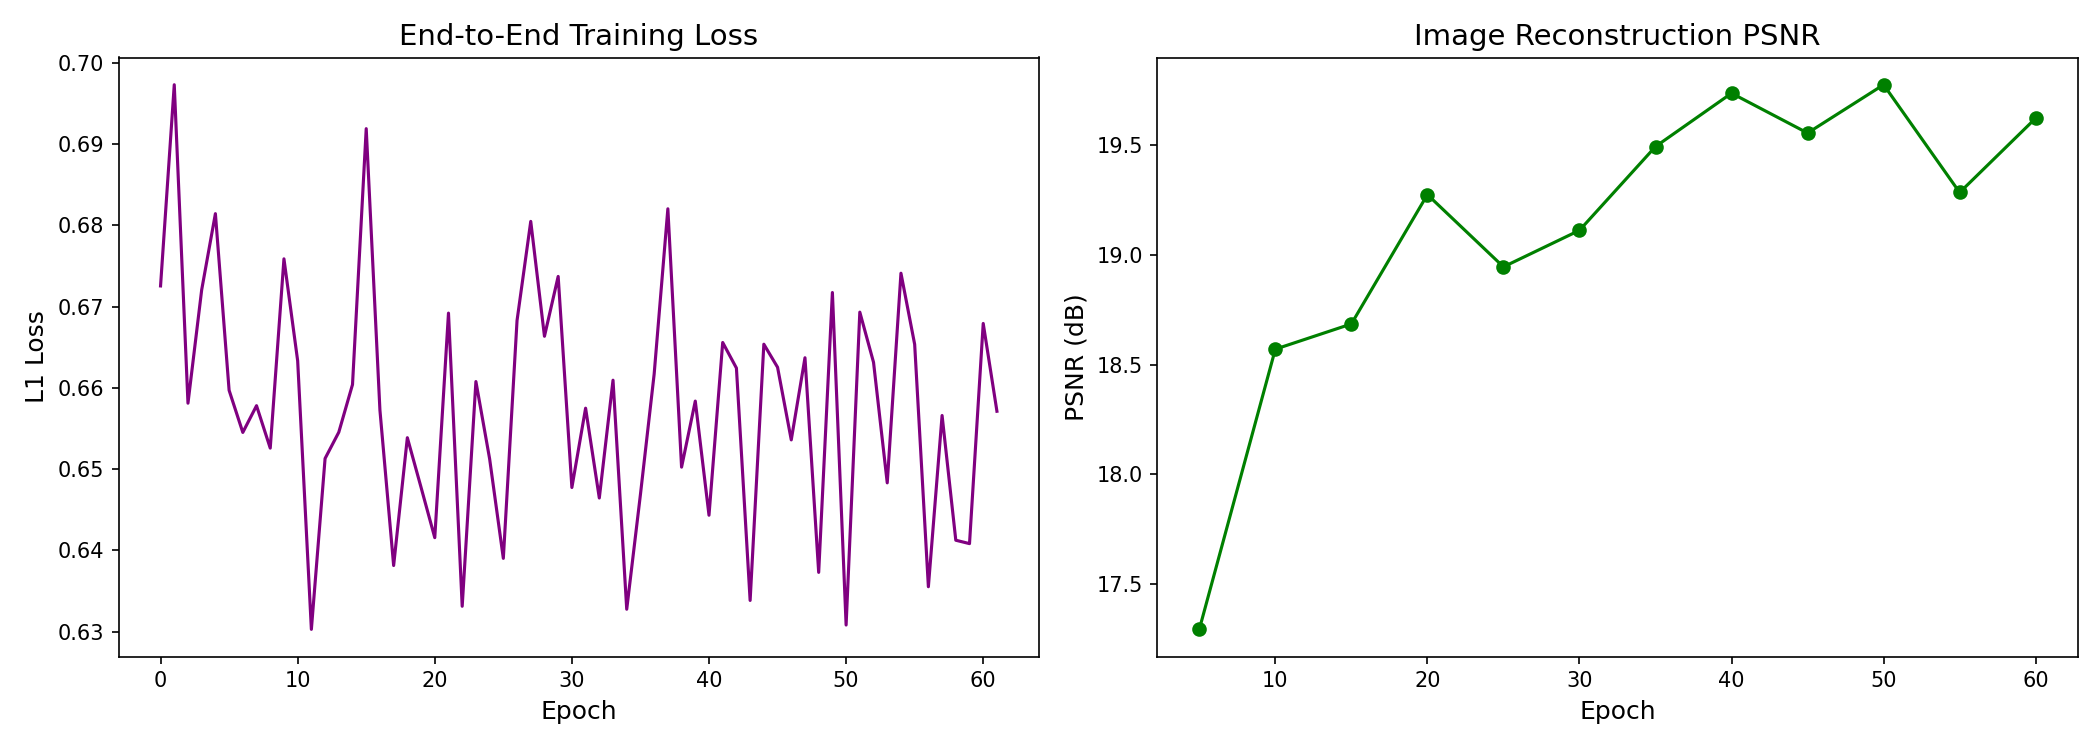
\includegraphics[width=0.78\textwidth]{figures/e2e_training_curves.png}
\caption{端到端训练曲线（PSNR/Loss，tutorial\_0207-184619）}
\end{figure}

\begin{figure}[H]
\centering
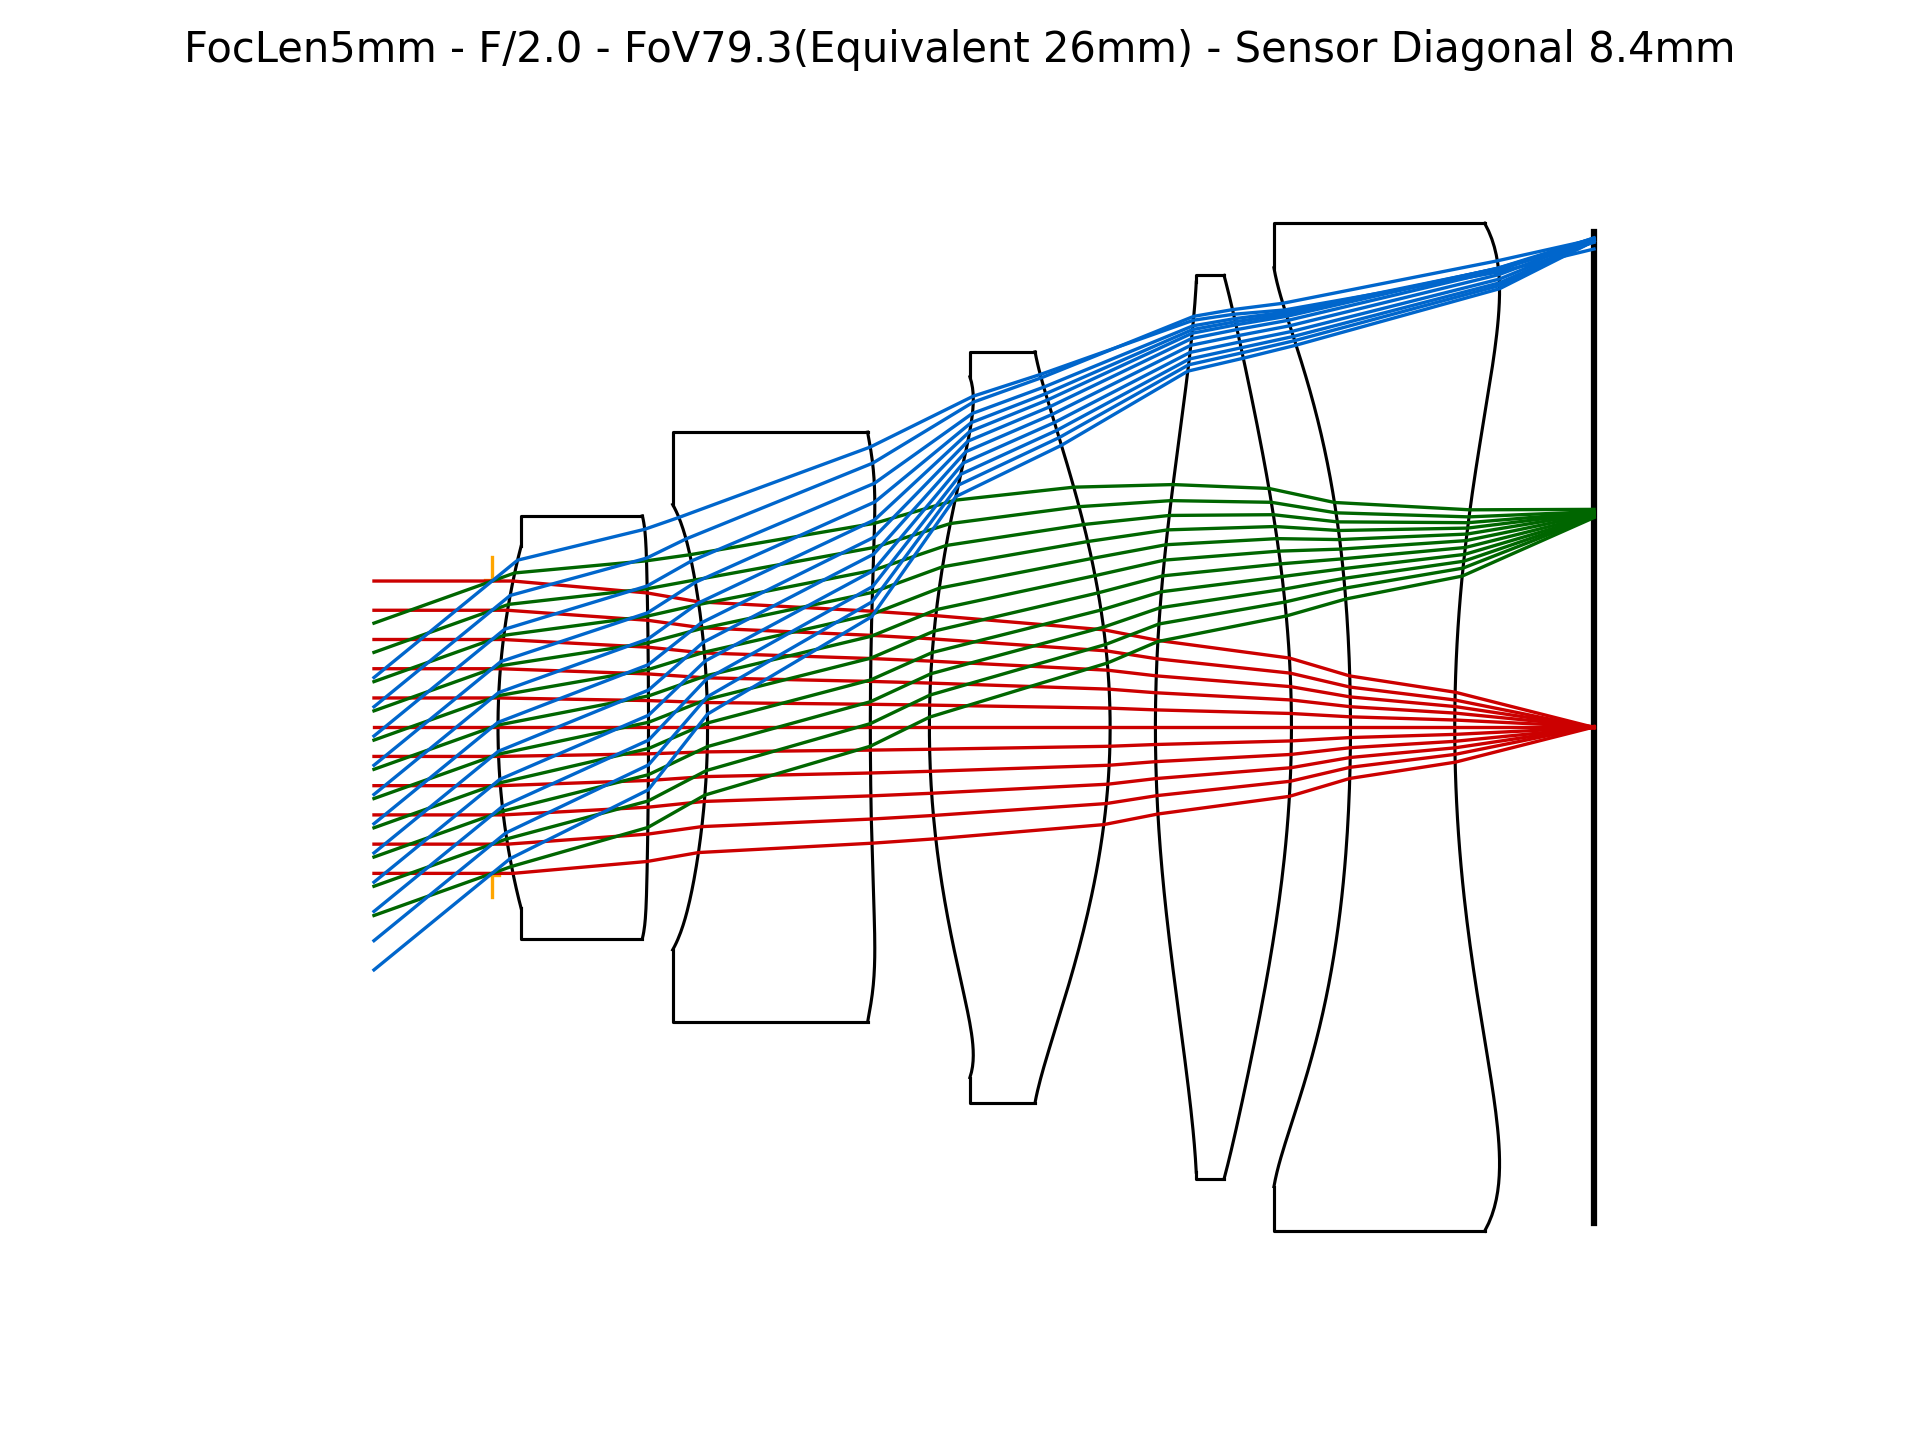
\includegraphics[width=0.78\textwidth]{figures/geolens_final_analysis.png}
\caption{折射系统综合分析图（tutorial\_0207-184619）}
\end{figure}

\begin{figure}[H]
\centering
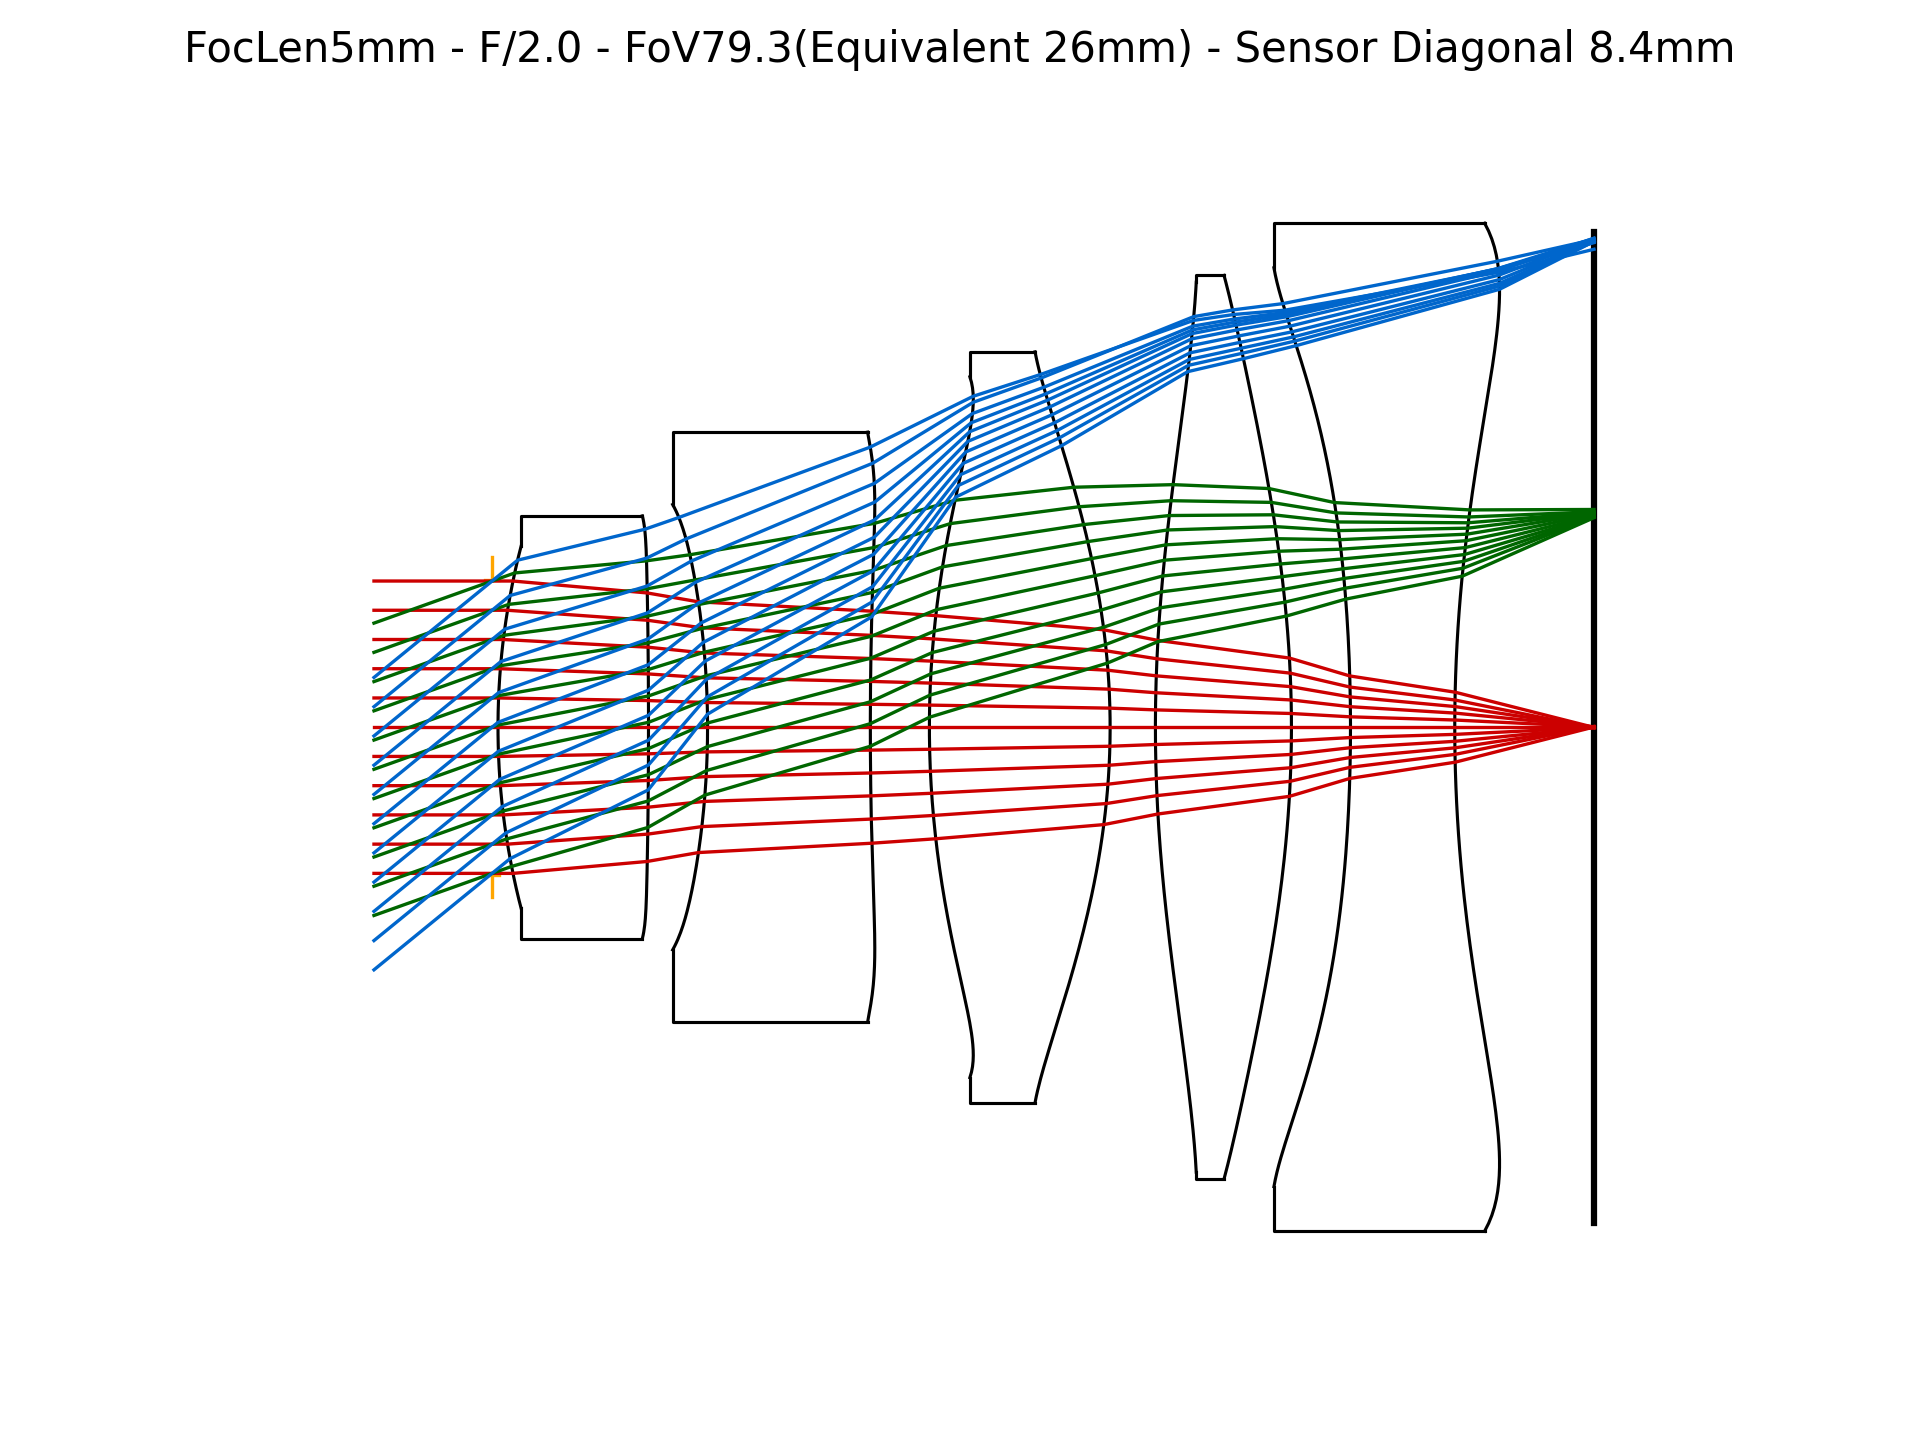
\includegraphics[width=0.78\textwidth]{figures/geolens_test.png}
\caption{独立测试折射分析图（standalone\_test\_0207）}
\end{figure}

\begin{figure}[H]
\centering
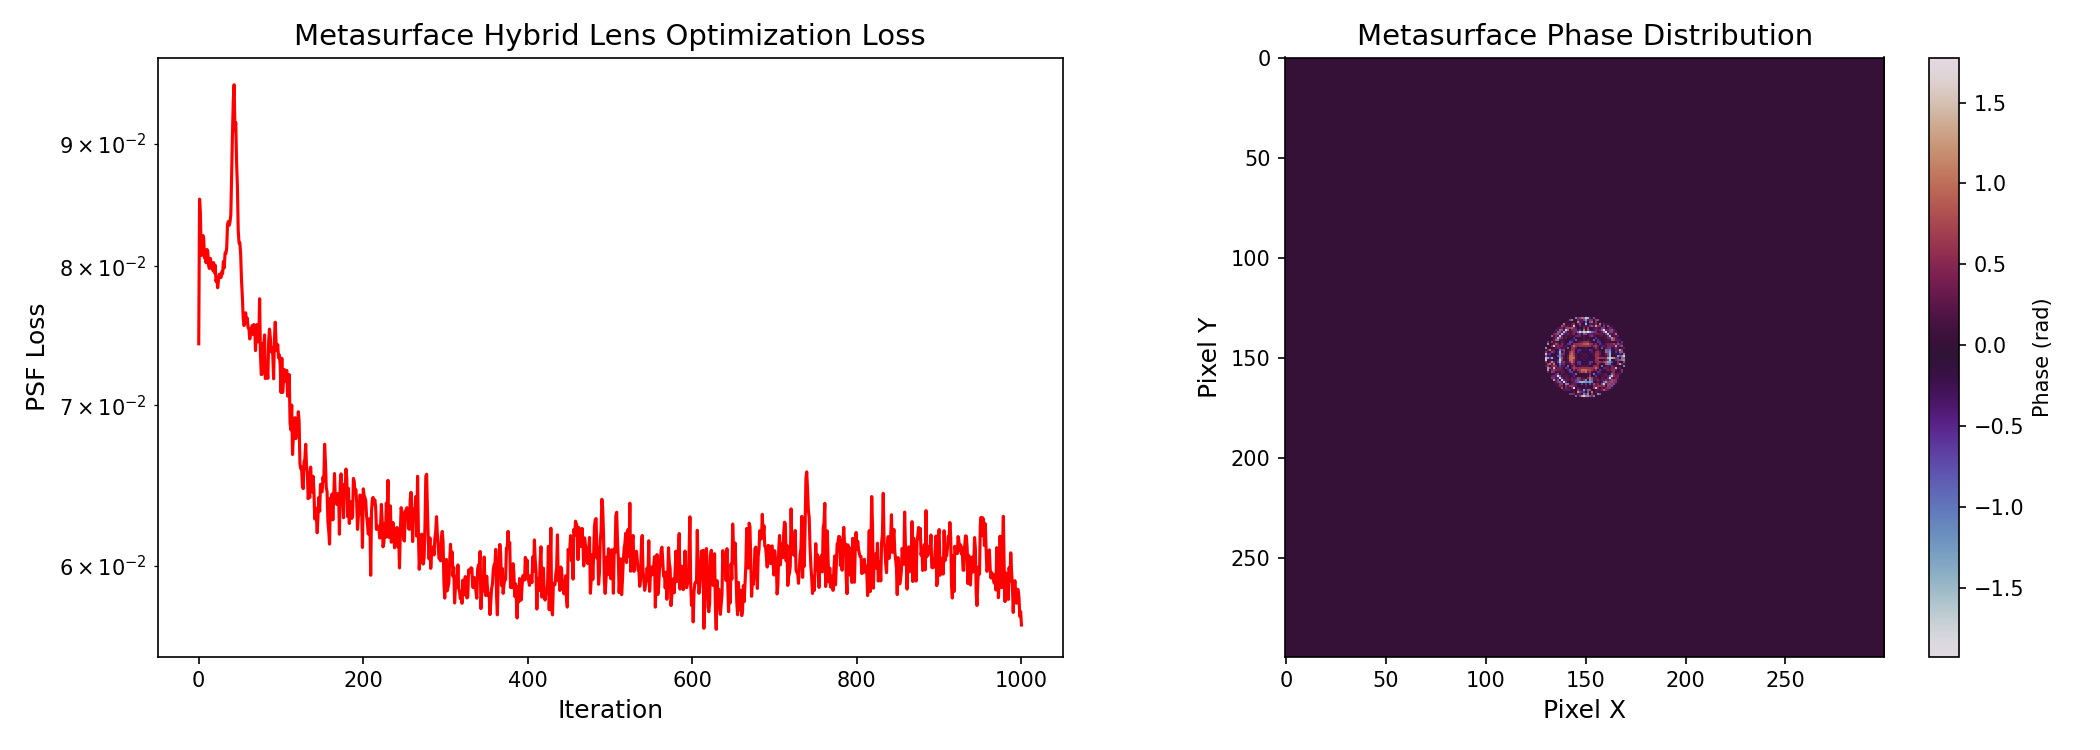
\includegraphics[width=0.78\textwidth]{figures/meta_optimization_results.png}
\caption{超表面扩展优化结果（tutorial\_0207-184619）}
\end{figure}

结合本轮日志可提取的定量结果，阶段结论可进一步细化为：第一，折衍混合优化在当前设置下由初始损失0.026145下降到0.014280，降幅45.4\%；第二，端到端训练在已记录轮次中PSNR由17.30dB提升至19.62dB，证明光学前端与重建网络联合训练链路有效；第三，独立测试目录已形成几何光学与重建三联样例，支持“训练结果可在独立流程下复核”的中期论证需求。需要强调的是，上述数值均为当前版本的阶段性统计，不等价于最终收敛上限，后续仍需在锁参后进行重复试验与显著性分析。

\hfirst{1.5 结果分析与阶段判断}
从工程可靠性看，当前最大成果是把“概念可行”转化为“流程可执行”。在以往仅有方法设想的阶段，研究风险主要来自不可实现性；而当前阶段风险已转化为参数优化和实验组织问题，这意味着项目已经跨过实现门槛。具体表现为：其一，代码结构清晰，配置驱动实验可复现；其二，图像证据链完整，可支撑中期答辩；其三，问题边界明确，后续任务可量化。

从学术严谨性看，当前工作坚持不夸大结论，明确区分已完成、进行中和待完成事项。已完成内容包括流程实现与预实验；进行中内容包括参数定型与端到端主指标评估；待完成内容包括超表面扩展对照、统计显著性分析与失败案例体系化归纳。该分层表达符合中期报告应有的证据强度要求。

从方法价值看，分阶段路线在当前任务上是有效的。若直接做全链路联合优化，训练不稳定风险较高；通过先建立折射基线再引入DOE，再引入重建网络，可以逐步控制复杂度，并在每一层获取可解释中间结果。这些中间结果不仅用于调试，也用于论文论证中的因果链构建。

\hfirst{1.6 文字化成果总结}
本课题中期阶段的核心成果可以概括为四点。第一，形成了可微分射线-波动联合建模的工程实现路径。第二，构建了从折射到折衍混合的稳定训练流程。第三，建立了面向图像与光学双域的评估框架。第四，完成了报告与展示材料的模板化迁移基础。上述成果为后续冲刺阶段提供了稳定起点。

同时，本课题已建立基本的质量控制机制：每次关键实验保留配置快照、日志文件和结果图，避免“无法复现的好结果”；每次结论输出前检查是否存在越界推断；每次版本更新后进行编译和图表引用检查，确保文档工程质量。该机制是毕业设计后半程保持节奏和质量的关键保障。

\hfirst{1.7 可微分射线-波动联合模型的技术细化说明}

为确保模型叙述具备审查可读性，本节对射线段、波动段和耦合段进行独立说明。射线段采用多场点光线采样并进行界面交点求解，核心目标是高效得到光线在DOE平面的入射位置、方向和相位参考项。交点计算采用可微分求解策略，在训练中保留对曲率、厚度和非球面系数的梯度通道。波动段采用标量衍射近似进行传播，输入为DOE调制后的复振幅，输出为像面复场，再由模平方得到PSF。耦合段的关键是坐标一致性和能量归一化一致性，如果在此处处理不当，训练会出现梯度方向失真，即损失下降但图像质量不提升。



在实现过程中，为减小内存开销并保持梯度稳定，课题采用“逐波长独立传播、后融合”的策略。即先分别计算RGB波段PSF，再根据传感器响应进行加权组合。该策略相较于一次性多波长联算更易控制显存峰值，也便于定位某一波段导致的异常收敛现象。对于波动传播过程，课题在中期阶段主要采用固定采样网格，并通过实验对比不同网格尺寸的稳定性收益。结果表明，在当前参数范围内，中等网格可兼顾速度与保真度，适合作为主实验默认设置。



模型数值稳定性的另一个关键点是归一化策略。PSF若不做稳定归一化，训练中容易出现“亮度漂移主导损失”的问题，导致系统倾向于通过能量缩放而非光学优化来降低误差。为此，本课题在每次PSF生成后执行一致归一化，同时在损失项中保留结构性约束，确保优化方向指向像质改善而非数值投机。该处理在中期预实验中已验证可显著减小训练曲线抖动。



\hfirst{1.8 端到端训练机制与数据流程说明}

端到端阶段的数据流由四个步骤构成。第一步，输入清晰图像通过光学退化模型生成退化观测；第二步，退化观测输入重建网络得到恢复图像；第三步，计算PSNR主损失及辅助结构损失；第四步，将损失反向传播到网络参数和光学参数。该流程的难点在于不同模块的梯度量级差异：网络参数更新通常更快，光学参数更新相对慢且噪声大。若不做分组学习率，系统容易出现“网络过拟合退化核、光学参数几乎不动”的现象，最终导致端到端收益有限。



为解决该问题，本课题采用分组优化器并在训练早期设置冻结策略。具体做法是先冻结部分光学高敏参数，仅更新网络和低敏光学参数，待网络进入稳定区间后再逐步解冻全参数。该策略可防止训练初期梯度噪声直接冲击光学结构，提高系统整体可训练性。与此同时，课题在数据层执行统一预处理，包括尺寸规范化、颜色通道一致化和强度归一化，避免数据层不一致造成伪差异。



在评估流程上，端到端阶段不只报告单次最好结果，而是报告多次重复试验的平均值和标准差。这样可以反映训练随机性对结果的影响，避免“一次偶然最好值”误导结论。对于视觉展示，采用同一批样本进行跨方案比较，并固定可视化参数，确保图像对比公平。所有可视化样本均保留源图、退化图和重建图三联图形式，便于答辩中直接说明误差来源。



\hfirst{1.9 折射、DOE与超表面路径的比较逻辑}

中期阶段已确认先DOE后超表面的推进顺序，其原因并非偏好，而是由任务约束决定。DOE路径参数维度较低、优化收敛更快，适合作为主线建立定量证据；超表面路径参数自由度更高、表达能力更强，但训练开销更大、稳定性更敏感，适合在主线稳定后作为扩展验证。通过该顺序安排，可以在有限周期内同时兼顾主线结果交付和方法上界探索。



从模型层看，DOE多项式参数化在可解释性方面有优势。参数变化可直观映射到相位轮廓变化，便于分析“参数-像质”关系；超表面像素参数化更接近自由形状优化，虽然潜在性能更高，但可解释性较弱。论文论证中，主线需要稳定可解释证据，因此优先DOE；扩展章节可展示超表面潜力及其工程代价，从而形成完整论证链条。



从工程层看，DOE路径更适合做参数扫描和消融试验。其训练速度和存储需求可控，便于在统一预算下开展多组对比。超表面路径在中期阶段若作为主线，容易因资源压力导致对比组数量不足，进而影响统计可靠性。因此当前策略强调“先确保主线证据完整，再做高自由度扩展”，该策略与毕业设计的时间和资源约束一致。



\hfirst{1.10 实验规范、统计约束与论证边界}

为保证最终结论可审核，本课题制定了统一实验规范。其一，所有主实验共享数据划分、训练轮次、随机种子管理规则和评估脚本。其二，任何参数改动必须记录变更原因和影响范围。其三，所有对比图表均注明实验版本和配置编号，防止结果错配。该规范的目标是将“研究行为”转化为“可审计流程”，从源头降低结论争议。



统计约束方面，主结果至少三次重复并报告均值和标准差。若两方案均值差异低于随机波动尺度，不给出强优劣判断，而是归类为“差异不显著”。该处理符合学术审稿对结论强度的要求。对于失败实验，本课题不做删减展示，而是记录失败条件、现象、修复尝试与未解决问题。负结果记录有助于解释方法边界，也可证明研究过程的真实性。



论证边界方面，本报告坚持三条原则。第一，只对已完成实验给出确定性结论；第二，对进行中工作只给阶段判断，不外推最终性能；第三，对待完成工作只陈述计划与可验证指标，不预置结论。通过边界约束，报告可以在保持信息充分的同时避免结论越界，从而满足中期评审对严谨性的核心要求。



在文档工程层面，课题同步执行格式一致性检查，包括页边距、标题风格、图题样式、段落行距、引用格式与图表编号。该检查不仅服务视觉规范，也直接关系答辩表达效率：当文档结构清晰、证据路径明确时，评审能够更快定位关键结论，提高沟通效率。中期模板迁移工作的意义正在于此，即把技术内容与规范表达统一到同一交付标准下。

\hfirst{1.11 新结果定量映射与证据闭环}

为避免“有图无数”或“有数无证”的断裂叙述，本稿对新结果建立了定量映射关系。映射的第一层是配置与结构参数：从\texttt{e2e\_epoch60.json}、\texttt{hybrid\_final.json}、\texttt{metalens\_final.json}可提取焦距、光圈数、传感器尺寸、像面距离与DOE配置字段；该层用于回答系统“设计到了什么状态”。映射的第二层是优化过程参数：从notebook日志可提取\texttt{hybrid\_iterations=3000}、\texttt{e2e\_epochs=1000（计划）}、\texttt{e2e\_lr\_net=1e-4}、\texttt{e2e\_lr\_doe=0.01}、\texttt{doe\_lr=0.1}等；该层用于回答系统“如何训练到该状态”。映射的第三层是性能与稳定性参数：从日志中提取Stage 1 improvement 25.4\%、Hybrid loss improvement 45.4\%、E2E PSNR提升轨迹；该层用于回答系统“训练是否产生可解释收益”。

在此基础上，本稿构建“图-表-文三向一致”规则。图像层提供直观变化证据，例如折射结构图、MTF/Spot图、DOE相位图、损失曲线、端到端训练曲线。表述层负责声明每个图像对应的实验目录和阶段目标，避免跨目录误配。结论层只对可追溯数据给出确定语句，对未完成统计显著性验证的项保持审慎用语。该规则可以防止中期报告常见的两类问题：一类是把单次最优值写成总体规律，另一类是图像和文字来自不同训练版本导致的逻辑冲突。

进一步地，为保证答辩中的可追问性，本稿将每类结论都绑定可复查路径。若评审追问“端到端结论依据是什么”，可对应到\texttt{e2e\_training\_curves.png}及notebook中Epoch日志；若追问“折衍混合是否真正收敛”，可对应到\texttt{hybrid\_loss\_curve.png}及\texttt{hybrid\_iter*.json}序列；若追问“扩展方向是否只停留在口头”，可对应到\texttt{meta\_optimization\_results.png}与\texttt{meta\_iter*.json}。通过路径绑定，报告从叙述文档转化为可审计文档，这也是中期阶段确保严谨性的关键举措。

最后，本稿针对“进行中”状态给出明确边界。端到端部分虽已出现PSNR提升趋势，但尚未完成多随机种子重复和全指标联合统计，因此不宣称最终最优结论。超表面扩展部分虽已形成可视化优化结果，但尚未在统一预算下完成与DOE主线的公平对比，因此仍定义为扩展验证阶段。上述边界定义并非降低结论力度，而是通过明确证据强度来提升结论可信度，符合中期报告的评审逻辑和学术规范。

为进一步保证后续终稿质量，本课题同时建立“写作前校验清单”。清单包含五项：第一，任何数值都必须在日志或结果文件中定位到来源；第二，任何图像都必须标注实验目录和阶段；第三，任何结论都必须给出边界条件；第四，任何对比都必须说明是否在统一预算下完成；第五，任何异常都必须在附录中保留记录。该清单将作为中后期写作与答辩准备的统一执行标准，确保论文不仅有结果，还具备过程透明性与结论可复核性。


\section*{二、存在的问题和拟解决方案}

\hfirst{2.1 存在的问题}
\subh{（1）参数定型尚未完全收敛。}
焦距、F数、厚度预算、DOE位置和采样密度之间存在耦合。当前虽然已有可用候选方案，但尚未完成统一预算下的最终收敛。若在此阶段直接下结论，可能导致后续结果解释出现偏差。

\subh{（2）端到端主指标体系仍需补齐。}
你已明确后续混合设计阶段以PSNR为主指标。当前端到端阶段已形成阶段性结果，日志显示PSNR从17.30dB提升至19.62dB，但尚未完成多随机种子重复、显著性检验与全量样本统计。因此SSIM与LPIPS仍需与PSNR联动分析，避免单指标偏置。

\subh{（3）高自由度相位参数导致训练稳定性压力。}
当DOE分辨率提高或扩展到Pixel2D超表面时，参数量显著增加，训练可能出现震荡、收敛变慢或局部最优。若学习率调度、正则化与采样设置不匹配，结果可能在不同随机种子下波动较大。

\subh{（4）计算资源约束与实验节奏存在冲突。}
大采样PSF和高分辨率相位传播会提高计算开销。在毕业设计时间窗口内，需要在“指标上限”和“实验可完成性”之间做可审计的平衡，否则容易出现实验计划延误。

\subh{（5）可制造性讨论仍偏弱。}
当前重点在仿真验证，制造可行性约束虽在正则项中有所体现，但尚未形成系统的容差分析和工艺边界讨论。若后续答辩问及工程落地，需要给出更明确的边界解释。

\hfirst{2.2 拟解决方案}
\subh{（1）建立统一参数收敛协议。}
采用“粗筛-精筛-锁定”三步法。粗筛阶段以低成本配置搜索候选区间；精筛阶段在固定预算下比较候选方案；锁定阶段冻结核心参数并用于全部主实验。每一步都记录配置与结果，保证可追溯。

\subh{（2）构建PSNR主导的多指标评估矩阵。}
以PSNR为主，SSIM和LPIPS为辅，并保留PSF、MTF、Spot等光学指标。报告方式采用“主指标提升+辅助指标一致性+可视化样例”三层结构。若主指标提升但辅助指标退化，按真实结果报告，不做选择性叙述。

\subh{（3）强化稳定训练策略。}
对折射参数、DOE参数、网络参数采用分组学习率；在阶段切换时引入冻结策略与warm-up；对高自由度相位参数加入平滑约束与梯度裁剪；必要时进行多次重复并报告均值和标准差，减少偶然性。

\subh{（4）实施资源受限下的分级实验。}
将实验分为探索级、验证级和汇报级。探索级用于快速定位趋势，验证级用于机制分析，汇报级用于最终结论。通过分级组织，在计算资源受限条件下确保关键结论按期产出。

\subh{（5）补充可制造性边界说明。}
在结果讨论中显式加入相位平滑度、结构尺寸、参数幅度等边界说明，明确“仿真可行”与“工程可制造”之间的距离，保证结论严谨。

\hfirst{2.3 风险闭环与质量控制}
为防止后续阶段出现“实验做了但结论不可信”的问题，本课题建立闭环机制：问题发现 $\rightarrow$ 原因定位 $\rightarrow$ 修复实验 $\rightarrow$ 对照验证 $\rightarrow$ 文档固化。每个环节均要求有证据输出。对于失败实验，不删除、不回避，统一归档并标注失败原因。该机制能够提升论文论证完整性，并减少答辩问答中的漏洞。

此外，文档层面采用“事实清单驱动写作”，确保每个结论都能追溯到图表或日志。对于未完成事项，统一使用“待验证”表述，不使用“已证明”表述。通过这种约束，可以在保持文字严谨的同时降低结论越界风险。

\hfirst{2.4 关键技术问题的深化分析}
当前最需要持续跟踪的技术问题是“光学优化目标”和“图像重建目标”之间的耦合关系。若仅强调光学指标，可能得到在点扩散层面良好但重建收益有限的结果；若仅强调图像指标，可能出现网络补偿掩盖光学缺陷的情况。为此，后续将采用双约束分析：一方面评估PSF、MTF、Spot随训练阶段的变化，另一方面同步评估PSNR、SSIM和LPIPS，并观察二者是否一致改进。若出现冲突，则通过损失项重加权和冻结策略调整优化方向。

第二个技术问题是跨场点一致性。当前结果在中心视场已具备较好稳定性，但离轴区域仍是性能波动的主要来源。离轴问题通常由两类因素叠加：一类是物理建模近似误差，另一类是训练样本覆盖不足。针对前者，后续将增加离轴场点权重并复核传播近似条件；针对后者，将在训练和验证样本中提高边缘场景占比，确保模型不会“只优化中心，不优化边缘”。该策略能够增强结论在实际应用场景中的可信度。

第三个技术问题是相位参数的可解释性。高自由度相位参数虽然有潜在性能优势，但若缺乏约束，容易出现局部高频振荡，导致结果难以解释且制造风险增大。后续将通过平滑正则和幅度边界对相位参数进行控制，并在论文中给出“参数分布-成像变化”的对应分析图。通过可解释性约束，可以把“性能提升”与“结构合理”同时纳入评价标准，避免得到不可落地的最优解。

第四个技术问题是结果稳健性。单次训练结果即使数值较好，也不能直接作为最终结论。后续将重点执行重复实验和扰动实验，包括随机种子扰动、轻微参数扰动和噪声水平扰动，观察结果是否保持同一趋势。若某方案在小扰动下性能剧烈波动，则不作为主结论方案。该机制可确保最终提交的结论具有工程可依赖性，而不仅是一次性最优展示。

第五个技术问题是跨阶段指标口径统一。中期阶段包含折射、折衍和端到端三个不同优化语境，若各阶段采用不同口径描述结果，会造成读者理解断裂。后续将统一指标口径和符号定义，例如将“阶段内最优”“阶段终点值”“全流程最终值”分别明确命名，并在图表中统一标注。这样可以确保论文中的纵向比较真实有效，避免因统计口径不一致造成伪提升。同时，所有关键结论都将附带对应实验编号，保证评审在追问时可快速定位原始证据。

第六个技术问题是图表语义一致性。当前图像数量较多，若图题、坐标轴和正文术语不统一，会降低报告可读性。后续将统一图题模板、坐标命名和单位表达，确保“同一指标在不同章节的写法一致”。该工作虽然不直接提升模型性能，但直接提升文档严谨性和答辩沟通效率。

同时将建立术语对照表，统一英文缩写、中文译名和符号含义，避免跨章节理解歧义。
并在附录中给出符号索引表。

\section*{三、下一步研究任务与进度安排}

\hfirst{3.1 研究任务分解}
下一阶段任务按“参数定型、主线实验、扩展实验、论文收敛”四块推进。

\subh{任务A：参数定型与折射基线重训。}
目标是锁定焦距、F数、厚度预算和采样设置，输出可复现基线。产物包括：正式配置文件、折射评估图、参数比较表。

\subh{任务B：折衍混合正式实验。}
在锁定参数下完成折射+DOE联合优化，补齐PSF、MTF、Spot和图像指标对比。产物包括：混合系统正式结果图、主对比表、误差分析段落。

\subh{任务C：端到端联合优化。}
完成混合光学前端与UNet联合训练，建立PSNR主指标结果，补充SSIM与LPIPS。产物包括：端到端训练日志、指标统计表、可视化案例。

\subh{任务D：超表面扩展验证。}
将DOE路径扩展到Pixel2D超表面，评估在更高自由度条件下的收益与代价。产物包括：扩展实验结果、复杂度分析、边界讨论。

\subh{任务E：论文与答辩材料收敛。}
完成最终论文正文、图表清单、参考文献校核和答辩PPT。产物包括：定稿论文、答辩演示文稿和问题清单。

\hfirst{3.2 进度安排（中期后）}
\begin{longtable}{p{3.2cm}p{10.2cm}}
\toprule
时间阶段 & 主要工作与验收标准 \\
\midrule
第1阶段（参数定型） & 完成候选参数对比，形成锁定参数集；验收标准为配置固定、基线结果可复现。 \\
第2阶段（折衍主实验） & 完成DOE联合优化正式训练与对照分析；验收标准为主对比图表齐全、结论边界清晰。 \\
第3阶段（端到端评估） & 完成PSNR主指标评估与辅助指标分析；验收标准为统计结果完整、可视化可解释。 \\
第4阶段（扩展与收敛） & 完成超表面扩展、失败案例整理、论文图表统一和答辩材料定稿；验收标准为文档可编译、图表可追溯、表达一致。 \\
\bottomrule
\end{longtable}

\hfirst{3.3 验收标准与交付清单}
为保证后续工作可管理，设定统一验收标准。

第一，实验验收：配置可复现、日志可追溯、指标可核算。第二，文档验收：图文一致、引用完整、结论不越界。第三，展示验收：叙事连贯、时间可控、问题边界清晰。交付清单包括：\texttt{midterm\_report.tex}、可选编译PDF、模板风格PPT、结果图目录与关键配置快照。所有交付项均需版本可追踪。

\hfirst{3.4 预期成果与完成判据}
后续完成判据不以单一指标为唯一标准，而是以“结果质量+证据完整度+可复现性”三项共同判定。预期成果包括：

1）形成一套可复现的端到端折衍混合设计流程；
2）给出折射、折衍混合、端到端和超表面扩展的系统对比；
3）形成主结果、消融实验与失败案例三类证据；
4）完成符合模板规范与学术规范的毕业论文正文和答辩材料。

若上述四项均达成，即可认为课题从“中期可行性验证”进入“终期定量结论交付”阶段。

\hfirst{3.5 主实验矩阵与消融试验安排}
为确保最终结论具有可审查性，后续实验将采用“主实验矩阵+消融实验矩阵”双线并行策略。主实验矩阵用于回答“哪种系统方案更有效”，消融实验矩阵用于回答“性能增益来自哪个机制”。主实验矩阵固定四个方案：纯折射基线、折射+DOE、折射+DOE+UNet、折射+超表面扩展；所有方案在同一数据划分、同一训练预算、同一评估脚本下执行。消融实验矩阵重点覆盖四个因素：课程学习调度、损失权重组合、相位正则化强度、采样密度与PSF核尺寸。通过该设计，可以在结果层和机理层同时给出证据。

每个主实验均至少重复三次，记录平均值和标准差。为避免“对比不公平”，所有方案都采用一致的硬件时间预算上限；若某方案因资源限制必须下调采样密度，将在结果表中单独标注，并在讨论中说明潜在影响，不将其与满预算方案做直接优劣判断。每轮实验结束后，先做自动化指标汇总，再做人审抽样，确认图像质量与指标走势一致。若出现指标提升但视觉退化的情况，按“指标冲突样本”归档并进入下一轮误差定位。

在消融试验中，坚持单变量控制原则。即每次仅改变一个因素，其余配置保持不变。对于不稳定现象（如同配置多次结果波动较大），不直接判定方法失效，而是追加“稳定性复验组”：固定随机种子、固定数据顺序、固定学习率，再观察是否仍存在异常。若异常消失，则归因于随机扰动；若异常持续，则归因于模型或损失设计问题。该流程可以显著降低误判风险。

\hfirst{3.6 数据治理、版本管理与可复现机制}
中后期阶段将把“实验可复现”作为与“结果提升”同等重要的目标。数据治理方面，训练集、验证集、测试集采用固定索引文件管理，不允许在实验中临时变更样本边界。所有图像预处理流程以脚本化方式固化，禁止手工预处理进入主实验。版本管理方面，每组实验建立唯一实验编号，绑定配置文件哈希、代码提交版本、模型输出路径和日志文件。任何结果图都必须可追溯到对应实验编号，避免后期论文整理时出现“图与配置不一致”的风险。

日志字段将统一为基础信息、训练信息、评估信息和异常信息四类。基础信息包含日期、设备、随机种子、数据版本；训练信息包含学习率、损失项、迭代计数、阶段切换点；评估信息包含PSNR、SSIM、LPIPS和光学指标；异常信息包含显存溢出、梯度爆炸、收敛中断等事件。每个实验结束后自动生成摘要报告，摘要至少包含三部分：关键指标表、训练曲线图、失败样本链接。该机制可以把繁杂日志转换为可答辩的证据资产。

为减少论文后期返工，后续将执行“图表先行”的文档策略。即在完成每组核心实验后立即产出对应图表和图注初稿，再由正文对图表做解释。这样可以保证论文叙事顺序与实验真实顺序一致，避免“先写结论后补证据”的写作风险。对于未达预期结果，照常进入图表库并标注“负结果”，不进行删除和隐藏。负结果记录不仅有助于内部调试，也能在论文中体现研究诚实性和方法边界。

\hfirst{3.7 风险分级与应急策略}
后续执行期将风险分为三级。一级风险为可快速修复问题，例如路径配置错误、单次训练中断、图像导出异常；二级风险为影响阶段进度的问题，例如参数长期不收敛、关键指标提升不足、实验预算超时；三级风险为影响最终交付的问题，例如核心主线无法形成统计显著差异、扩展实验无法完成、文档结构与证据不一致。针对一级风险，采用当日修复机制；针对二级风险，采用周度复盘机制；针对三级风险，采用里程碑重规划机制。

在应急策略上，设置“保底主线”与“增强扩展”两套方案。保底主线保证折射与DOE主结果完整可交付，即使扩展路径受阻，仍可形成合格毕业论文；增强扩展用于在资源允许时推进超表面和更多消融。该双路径机制可防止项目被单一高风险任务拖累，确保在最坏情况下仍能完成核心成果交付。

当出现关键指标停滞时，优先按“数据、损失、优化器、模型、资源”顺序排查。先确认数据流程无误，再检查损失权重是否失衡，再验证学习率和冻结策略是否合理，最后评估模型复杂度与资源是否匹配。排查过程要求逐步单变量，避免多变量同时调整导致原因不可定位。每次排查必须有记录并形成结论，确保团队协作和个人回溯时信息完整。

\hfirst{3.8 预期学术贡献与工程贡献}
从学术角度，课题预期贡献在于提供一套可复现的分阶段折衍混合优化路径，并通过统一评估协议给出可审查的对比证据。与仅报告单一最优结果的工作不同，本课题强调“结果+机制+边界”三位一体论证：既报告性能变化，也解释变化原因，还说明方法适用边界。该论证方式有助于提高结论可信度，并为后续相关研究提供可直接借鉴的实验范式。

从工程角度，课题预期贡献在于形成可长期复用的项目资产，包括配置模板、训练脚本、评估脚本、图表生成流程和文档模板。这些资产能够支持后续迭代，而不仅服务一次性答辩。特别是模板化文档体系的建立，使“技术输出”和“规范输出”在同一流程中完成，减少了研究后期因格式返工造成的时间损耗。

在人才培养层面，课题将把“严谨表达”纳入技术能力的一部分。即不仅追求模型效果，还要求结论表达可核验、图文一致、边界清晰。该能力对于后续继续深造或进入工程岗位都具有直接价值。通过本阶段的规范化推进，预期可形成一份同时满足技术深度与文档规范的毕业设计成果。

\hfirst{3.9 论文定稿阶段的证据组织方案}
为保证终稿答辩时能够在有限时间内完成有效沟通，论文证据组织将采用“主结论先行，证据逐层展开”的编排方式。第一层为主结论表，集中呈现各方案核心指标及统计范围。第二层为机制解释图，说明折射参数、相位参数和网络参数分别带来的变化。第三层为边界与负结果，展示在何种条件下方法增益减弱或失效。通过三层结构，读者可以先看到“是否有效”，再看到“为什么有效”，最后看到“何时失效”，避免单向度叙述导致的可信度下降。

在图表布局上，终稿将统一采用“结论图+解释图+失败图”三联结构。结论图用于展示指标对比，解释图用于呈现相位图、PSF或误差曲线变化，失败图用于说明当前方法边界。每组图表均附带配置编号、随机种子范围和训练预算信息，确保图与文可回溯。对于公式推导部分，不追求冗长推演，而强调“定义完整、符号统一、与实现一致”。若某变量在代码中有不同命名，需在文中给出对应关系，避免评审质疑理论与工程脱节。

终稿写作阶段还将进行两轮交叉审读。第一轮检查事实准确性：图表是否来自对应实验，引用是否对应，结论是否超出证据。第二轮检查表达一致性：术语是否统一，章节之间是否存在重复或冲突，是否存在口语化和模糊表述。每轮审读后形成问题清单并逐项关闭。该流程可显著降低“技术正确但文档不严谨”的风险。

\hfirst{3.10 答辩准备与问答预案}
答辩准备按“问题清单驱动”方式开展，重点覆盖四类高频问题。第一类是方法合理性问题，例如为何采用分阶段路线而非一次性联合优化。第二类是结果可信度问题，例如是否存在挑选样本、是否做了重复实验。第三类是工程可行性问题，例如训练资源需求、参数可制造性、部署复杂度。第四类是扩展能力问题，例如超表面路径是否具备现实收益、后续是否可迁移到其他成像任务。

针对上述问题，预案将统一采用三句式回答：先给事实，再给原因，最后给边界。以“为何先DOE后超表面”为例，事实是DOE路径在当前预算下收敛更稳定；原因是参数维度更低、可解释性更强；边界是超表面在性能上限上可能更优，已纳入扩展计划。通过这种结构化回答，可在有限答辩时间内保持逻辑完整，减少被追问时的信息断层。

此外，答辩演示材料将严格对应论文章节，不出现“PPT有而论文没有”或“论文有而PPT缺失关键证据”的情况。每一页PPT都绑定论文中的具体图表或结论段落，并在演练稿中标注页码和问答补充点。对可能被追问的负结果，提前准备原因分析与后续改进路线，保持论证透明。该策略可有效提升答辩现场的稳定性与说服力。

\section*{四、指导教师意见（占位）}
本节按模板要求保留。待指导教师填写正式意见后，替换本占位文字。建议填写内容包括：

1）对研究内容完整性与技术路线合理性的评价；
2）对阶段成果真实性与可复现性的评价；
3）对存在问题及后续计划可执行性的建议；
4）对毕业设计后续重点工作的指导意见。

\section*{五、中期审核负责人意见（占位）}
本节按模板要求保留。待中期审核负责人填写正式意见后，替换本占位文字。建议填写内容包括：

1）对中期工作量与质量是否达到要求的结论；
2）对论文结构、表达规范、证据完整性的审核意见；
3）对后续整改事项和时间节点的明确要求。

\vspace{1.2em}

\noindent 参考文献：
\bibliographystyle{unsrt}
\bibliography{references}

\end{document}
